\documentclass[conference]{IEEEtran}
\usepackage{graphicx}
\IEEEoverridecommandlockouts
\usepackage{cite}
\usepackage[T2A,T1]{fontenc}
\usepackage{scn}
\usepackage{ulem}
\usepackage{amsmath, amssymb, amsfonts}
\usepackage{algorithmic}
\usepackage[utf8]{inputenc}
\usepackage[russian, english]{babel}
\usepackage{listings}
\usepackage{comment}
\usepackage{tikz}
\usepackage{pgfplots}
\pgfplotsset{compat=1.18}
\usepackage{metalogo}
\usepackage{adjustbox}

\usepackage[hyphens]{url}
\usepackage[colorlinks=true, linkcolor=blue, urlcolor=blue, citecolor=blue]{hyperref}
\usepackage{hyphenat}
\usepackage{balance}

% TikZ libraries for advanced diagrams
\usetikzlibrary{positioning, fit, calc, arrows.meta, patterns, shapes.geometric,
patterns.meta}

% For Cyrillic font substitution
\DeclareFontFamilySubstitution{T2A}{\rmdefault}{Tempora-TLF}

\selectlanguage{english}

\title{Neuro-symbolic controller for Pasteurizer}

\author{ \IEEEauthorblockN{Dzmitry Ivaniuk} \IEEEauthorblockA{JSC ``Savushkin
  Product'', Brest, Republic of Belarus\\
Email: Ivaniuk.Dzmitry@savushkin.com} }

\begin{document}

\maketitle

\begin{abstract}
  This article provides a review of the current state of neuro-symbolic AI and
  neuro-symbolic control systems in industry, and examines their application to
  a pasteurization controller based on OSTIS Technology, as well as their
  integration with classical approaches and standards in Industry 4.0, such as
  ISA-88, ISA-95, and ISA-5.1.
\end{abstract}

\begin{IEEEkeywords}
  Neuro-symbolic AI, neural network, ANN, reinforcement learning, standards,
  ontologies, Industry 4.0, Industry 5.0, OSTIS, ISA-88, ISA-95, ISA-5.1.
\end{IEEEkeywords}

\section{Introduction}

This paper builds upon the ideas discussed in
\cite{ivaniuk2025neurosymbolic,ivaniuk2024neurosemantic,Lutska2022,Taberko2020,
Golovko2018integration} and reviews current challenges and tools for developing
and applying industrial standards alongside modern techniques such as
neuro-control, \textbf{neuro-symbolic AI}, and semantic technologies. It also
summarizes the history of \textbf{SCADA} systems and their evolution into modern
control systems integrated with AI and Industry 4.0 technologies. The main focus
is on standards-related problems and their relevance to today's control systems.
A symbolic neurocontroller is presented as a promising approach for controlling
complex industrial processes such as pasteurization by combining the strengths
of symbolic and neural methods. Each level is governed by its own algorithms and
often resembles a black box: inputs and outputs are visible, while the internal
algorithm is hidden. For instance, a neural network can be represented as a
black box (Fig.~\ref{fig:black_nn}), but it remains important to understand the
underlying rules.

\begin{figure}[ht]
  \centering
  \begin{adjustbox}{width = \columnwidth}
    \begin{tikzpicture}


      % Draw the black box.
      \fill[black] (0,0) -- (2,0) -- (2,2) -- (0,2) -- cycle; % Front
      \fill[black] (2,0) -- (3,1) -- (3,3) -- (2,2);          % Right
      \fill[black] (0,2) -- (1,3) -- (3,3) -- (2,2) -- cycle; % Top

      % Draw the edges of the black box.
      \draw[thick, white] (0,0) -- (2,0) -- (2,2) -- (0,2) -- cycle; % Front
      \draw[thick, white] (2,0) -- (3,1) -- (3,3) -- (2,2);          % Right
      \draw[thick, white] (0,2) -- (1,3) -- (3,3);                   % Top

      % Draw a simple neural network on the front surface of the box.
      \node[draw=white, fill=white, circle] (in) at (0.2,1) {};
      \node[draw=white, fill=white, circle] (h1) at (1,1.5) {};
      \node[draw=white, fill=white, circle] (h2) at (1,1.1) {};
      \node[draw=white, fill=white, circle] (h3) at (1,0.7) {};
      \node[draw=white, fill=white, circle] (h4) at (1,0.3) {};
      \node[draw=white, fill=white, circle] (out) at (1.8,1) {};

      \draw[white, thick, ->] (in) -- (h1); \draw[white, thick, ->] (in) --
      (h2); \draw[white, thick, ->] (in) -- (h3); \draw[white, thick, ->] (in)
      -- (h4); \draw[white, thick, ->] (h1) -- (out); \draw[white, thick, ->]
      (h2) -- (out); \draw[white, thick, ->] (h3) -- (out); \draw[white, thick,
      ->] (h4) -- (out);

      % Draw the input arrow and text.
      \draw[thick, ->] (-1,1) -- (0,1); \node at (-1.5,1) {Inputs};

      % Draw the output arrow and text.
      \draw[thick, ->] (3,1) -- (3.9,1); \draw[white, thick, -] (2,1) -- (3,1);
      \node at (4.5,1) {Outputs};
    \end{tikzpicture}
  \end{adjustbox}

  \caption{Neural Network as a Black Box}
  \label{fig:black_nn}
\end{figure}

\section{History and background: from \texorpdfstring{\textbf{SCADA}}{SCADA} to
\texorpdfstring{\textbf{AI-aided control systems}}{AI-aided control systems}}

Supervisory Control and Data Acquisition (\textbf{SCADA}) systems have become
the backbone of modern industrial automation and control infrastructure. From
power generation and distribution to water treatment, oil and gas pipelines, and
manufacturing facilities, \textbf{SCADA} systems enable centralized monitoring
and control of geographically distributed processes.

Let us examine the evolution of \textbf{SCADA} systems over the past six decades
\cite{boyer2004scada,MFGTechHub2024,TechTarget2024}, tracing their development
from simple telemetry systems to sophisticated, networked control platforms.
Understanding this historical progression is essential for appreciating current
\textbf{SCADA} capabilities and anticipating future trends in industrial
automation.

The rapid pace of technological change in industrial control systems
necessitates a historical perspective to understand how \textbf{SCADA} systems
evolved to meet changing industrial needs, regulatory requirements, and
cybersecurity challenges.

\subsection{Pre-\textbf{SCADA} Era (Before 1960s)} Before the advent of
\textbf{SCADA} systems, industrial processes relied on manual monitoring and
control. Operators physically inspected equipment, read gauges, and manually
adjusted controls. This approach was labor-intensive, prone to human error, and
limited to small-scale operations.

\subsection{Birth of \textbf{SCADA} (1960s-1970s)} The first generation of
\textbf{SCADA} systems emerged in the 1960s as mainframe-based monolithic
systems. These early systems were characterized by:

\begin{itemize}
    \item \textbf{Centralized Architecture}: All processing occurred at a
    central mainframe computer
    \item \textbf{Proprietary Protocols}: Vendor-specific communication
    protocols with no standardization
    \item \textbf{Relay Logic}: Control based on relay circuits and hard-wired
    logic
    \item \textbf{Limited Connectivity}: Point-to-point connections using serial
    communication
    \item \textbf{Basic Telemetry}: Simple Remote Terminal Units for data
    collection
\end{itemize}

Several factors drove the development of early \textbf{SCADA} systems (Key
Drivers):
\begin{enumerate}
    \item Need for remote monitoring of geographically dispersed infrastructure
    \item Labor cost reduction through automation
    \item Improved safety through continuous monitoring
    \item Enhanced operational efficiency and response times
\end{enumerate}

\subsection{Second Generation: Distributed \textbf{SCADA} (1970s-1980s)} The
second generation introduced distributed computing concepts. Multiple computers
were networked using Local Area Networks (LANs), sharing control and monitoring
responsibilities. Key characteristics included:

\begin{itemize}
    \item Multiple systems performing similar functions
    \item Introduction of minicomputers
    \item LAN-based communication between systems
    \item Still largely proprietary protocols
    \item Improved redundancy and reliability
\end{itemize}

\subsection{Third Generation: Networked \textbf{SCADA} (1990s-2000s)} The third
generation marked a significant shift toward open systems and standard
protocols:

\begin{itemize}
    \item \textbf{Open Architecture}: Adoption of industry standards (e.g.,
    TCP/IP, Ethernet)
    \item \textbf{Standard Protocols}: Implementation of protocols like Modbus,
    DNP3, IEC 60870-5-104
    \item \textbf{Client-Server Model}: Separation of data acquisition and
    presentation layers
    \item \textbf{WAN Connectivity}: Wide Area Network communication enabled
    \item \textbf{COTS Components}: Use of Commercial Off-The-Shelf hardware and
    software
    \item \textbf{Human-Machine Interface (HMI)}: Advanced graphical user
    interfaces
\end{itemize}

\subsection{Fourth Generation: Internet of Things \textbf{SCADA}
(2010s-Present)} Modern \textbf{SCADA} systems integrate IoT technologies and
cloud computing:

\begin{itemize}
    \item Cloud-based \textbf{SCADA} platforms
    \item Big data analytics and machine learning integration
    \item Mobile device support for remote access
    \item Enhanced cybersecurity measures
    \item Edge computing capabilities
    \item Integration with Enterprise Resource Planning (ERP) systems
    \item Real-time data analytics and predictive maintenance
\end{itemize}


The evolution of SCADA has been closely tied to advances in communication
technology and hardware capabilities. As communication technologies evolved,
SCADA systems were able to expand their reach and functionality. The following
tables summarize the key communication technologies that have shaped SCADA
development over the years:

\begin{table}[h]
\centering
\caption{Evolution of SCADA Communication Technologies}
\label{tab:communication}
\begin{tabular}{@{}lll@{}} \textbf{Era} & \textbf{Technology} &
\textbf{Characteristics} \\
1960s--1970s & Serial/Analog Radio & Point-to-point, low bandwidth \\
1980s--1990s & Digital Radio & Improved reliability, bandwidth \\
1990s--2000s & Ethernet, TCP/IP & Standard protocols, LAN/WAN \\
2000s--2010s & Wireless, Cellular & Mobile connectivity, flexibility \\
2010s--Present & IoT, 5G, Satellite & High bandwidth, global coverage \\
\end{tabular}
\end{table}

\begin{table}[h]
  \centering
  \caption{Hardware evolution of SCADA systems}
  \label{tab:hardware_evolution}
  \begin{tabular}{@{}ll@{}} \textbf{Era} & \textbf{Key hardware} \\
    1960s--1970s & Mainframes, relay logic, basic RTUs \\
    1980s--1990s & Minicomputers, Programmable Logic Controllers (PLCs) \\
    1990s--2000s & Industrial PCs, advanced RTUs with local intelligence \\
    2000s--Present & Edge devices, IoT sensors, distributed processing units \\
  \end{tabular}
\end{table}

Software has been crucial to SCADA evolution:
\begin{itemize}
    \item Early proprietary software systems
    \item Introduction of databases for historical data storage
    \item Development of sophisticated HMI/SCADA software packages
    \item Web-based interfaces and mobile applications
    \item Integration with data analytics and AI platforms
\end{itemize}

Key protocols that shaped SCADA development include:
\begin{itemize}
    \item \textbf{Modbus} (1979): Simple master-slave protocol, still widely
    used
    \item \textbf{DNP3} (1993): Developed for electric utilities, robust and
    efficient
    \item \textbf{IEC 60870-5-104} (2000): International standard for power
    system control
    \item \textbf{OPC} (1996): Standardized data exchange between industrial
    systems
    \item \textbf{MQTT} (1999): Lightweight publish-subscribe protocol for IoT
    \item \textbf{OPC UA} (2006): OPC Unified Architecture
\end{itemize}

Modern SCADA systems are integral to the Fourth Industrial Revolution (Industry
4.0), characterized by:
\begin{itemize}
    \item Cyber-physical systems integration
    \item Internet of Things (IoT) connectivity
    \item Cloud computing and edge processing
    \item Big data analytics and artificial intelligence
    \item Digital twins for simulation and optimization
    \item Augmented reality for maintenance and training
    \item Cloud SCADA platforms
\end{itemize}

However, they also introduce concerns about data security, latency, and
reliability.

Modern SCADA systems leverage advanced analytics:
\begin{itemize}
    \item Predictive maintenance using machine learning algorithms
    \item Anomaly detection for early fault identification
    \item Process optimization through data-driven insights
    \item Energy consumption analysis and optimization
    \item Quality control through statistical process control
\end{itemize}

Despite standardization efforts, challenges remain: legacy systems using
proprietary protocols, integration of diverse vendor equipment, need for gateway
devices and protocol converters and ongoing standardization efforts (e.g., OPC
UA).

Many organizations face challenges in upgrading aging SCADA infrastructure:
\begin{itemize}
    \item High costs of replacement
    \item Risk of operational disruption
    \item Limited support for obsolete components
    \item Need for phased migration strategies
\end{itemize}

Several trends are shaping the future of SCADA:
\begin{itemize}
    \item \textbf{Edge Computing}: Processing data closer to sources for reduced
    latency
    \item \textbf{5G Networks}: Enabling real-time control over wireless
    networks
    \item \textbf{Blockchain}: For secure data exchange and audit trails
    \item \textbf{Digital Twins}: Virtual replicas for simulation and
    optimization
    \item \textbf{AI-Driven Automation}: Autonomous decision-making systems
    \item \textbf{Quantum Computing}: Potential for complex optimization
    problems
\end{itemize}


\section{AI and standards}

Although neural networks have given us many interesting developments,
researchers believe that for progress, AI must understand not only "what" but
also "why", that is, process cause-and-effect relationships. This has led to the
search for new directions in AI. Neuro-symbolic AI is a form of AI that combines
machine learning methods with symbolic systems.


Standardization describes different aspects of each developed human activity and
includes a system of concepts (including terminology), a typology, and a model
that describes how to apply appropriate methods and means, production sites,
types, and structures of project documents, and accompanying activities. The
existence of standards helps solve one of the key problems related to any
technology, particularly rapidly developing computer information technologies,
\textbf{compatibility problem} \cite{Golenkov2019}. Compatibility can be
analyzed from many aspects, from the consistency of terminology in the
interactions of process participants to the consistency of actions taken in the
process of technology application.

The cohesion of digital twin models is challenged by the need for many
disparate, unrelated, and heterogeneous models. On the other hand, connecting
digital twins in a single system \cite{DigitalTwins} requires interaction and
conceptual unification. It also requires SCADA systems to achieve higher levels
of integration, scalability, and technological modernity \cite{Mladen2022}.

Despite advances in information technology, most standards are now presented in
the form of traditional linear documents or web resources containing a series of
static pages connected by hyperlinks. This approach to expressing standards has
many serious drawbacks, and ultimately, the overhead costs of maintaining and
using standards outweigh their benefits \cite{Serenkov-2004}.

Recently, the development of semantic technologies has enabled the creation of a
new generation of standards based on formalized knowledge representation. These
standards allow for the creation of intelligent systems that can automatically
process and use this knowledge. This approach is based on the use of ontologies,
which are formal representations of knowledge in a specific domain, enabling the
creation of a common vocabulary and understanding of the concepts and
relationships within that domain \cite{Golenkov2019}.

\href{https://www.isa.org/}{ISA} (International Society of Automation) has
released Mimo: a large language model (LLM) specifically trained on ISA content
\cite{Mimo2024}, such as standards, technical reports, and other documents. It
is designed to assist users in understanding and applying ISA standards and
practices. Mimo can answer questions, provide explanations, and generate text
related to ISA content. It is intended to be a valuable resource for
professionals in the automation and control industry. Mimo is not a replacement
for human expertise but rather a tool to enhance understanding and application
of ISA standards.

However, the Mimo model is not open source and cannot be used in production. It
also cannot be integrated with other systems.

\section{Problems and state of the art}

An analysis of the work has made it possible to formulate the most important and
common problems related to the development and application of modern standards
in various fields \cite{Serenkov-2004, Uglev-2012}:

\begin{itemize}
  \item Above all, the complexity of maintaining the standards themselves due to
    the duplication of information, especially the complexity of changing
    terminology.
  \item Duplicate information in the documentation describing the standard.
  \item Standards internationalization issues — translating a standard into
    multiple languages actually requires supporting and coordinating independent
    versions of the standard in different languages.
  \item As a result, inconsistencies in the format of different standards. Also
    automating the process of developing and applying standards is complicated.
  \item The inconvenience of using the standard, especially the complexity of
    finding the information you need. As a result, the complexity of studying
    standards.
  \item The complexity of automating the verification that an object or process
    complies with the requirements of a particular standard.
  \item etc.
\end{itemize}

These problems are mainly related to the presentation of standards. The most
promising approach to solve these problems is the transformation of each
specific standard into a knowledge base, which is based on a set of ontologies
corresponding to this standard \cite{Golenkov2019, Serenkov-2004, Uglev-2012,
Improving-2017, ISA-88-formalization}. This approach allows us to significantly
automate the development processes of the standard and its application.

As an example, consider the \textbf{\textit{ISA-88}} \cite{ISA88} standard (the
basic standard for batch production). Although this standard is widely used by
American and European companies and is actively implemented on the territory of
the Republic of Belarus, it has a number of drawbacks. Essential ISA batch
systems standards are shown at Fig. \ref {fig:s88_parts}.

\begin{figure}[ht]
  \centering
  \begin{adjustbox}{width = \columnwidth}
    \begin{tikzpicture}[node distance=8mm and 18mm, every node/.style={draw, rounded corners, align=center, minimum width=26mm, minimum height=7mm, fill=blue!12}, arrow/.style={-Latex, thick}]
      \node[fill=blue!28] (root) {ISA-88}; \node[below=of root] (main)
      {88.00.01-2010}; \node[below left=of main] (sub1) {88.00.02-2001};
      \node[below right=of main] (sub2) {TR 88.00.02-2015}; \node[below=of sub2]
      (sub3) {TR 88.0.03-1996}; \node[below=of sub1] (sub4) {88.00.03-2003};
      \node[below left=of sub4] (sub5) {88.00.04-2006}; \node[below right=of
      sub4] (sub6) {TR 88.95.01-2008}; \node[below=of sub4] (sub7) {IEC
      61512-1\\GOST R IEC 61512-1-2016};

      \draw[arrow] (root) -- (main); \draw[arrow] (main) -- (sub1); \draw[arrow]
      (main) -- (sub2); \draw[arrow] (main) -- (sub3); \draw[arrow] (sub1) --
      (sub4); \draw[arrow] (sub4) -- (sub5); \draw[arrow] (sub4) -- (sub6);
      \draw[arrow] (sub4) -- (sub7);
    \end{tikzpicture}
  \end{adjustbox}
  \caption{ISA-88 parts as a hierarchical diagram}
  \label{fig:s88_parts}
\end{figure}

Another standard often used in the context of Industry 4.0 is
\textit{\textbf{ISA-95}} \cite{ISA95}. \textit{\textbf{ISA-95}} is an industry
standard for describing high-level control systems. Its main purpose is to
simplify the development of such systems, abstract from the hardware
implementation and provide a single interface to interact with the ERP and MES
layers. Consists of eight distinct sections, described at Fig. \ref
{fig:s95_parts}.

\begin{figure}[ht]
  \centering
  \begin{adjustbox}{width = \columnwidth}
    \begin{tikzpicture}[node distance=10mm and 20mm, every node/.style={draw, rounded corners, align=center, minimum width=28mm, minimum height=8mm, fill=green!12}, arrow/.style={-Latex, thick}]
      \node[fill=green!28] (root95) {ISA-95}; \node[below=of root95] (a)
      {95.00.01-2010}; \node[below left=of a] (b) {95.00.02-2018};
      \node[below=of a] (c) {95.00.03-2013}; \node[below right=of a] (d)
      {95.00.04-2018}; \node[below=of c] (e) {95.00.05-2018}; \node[below
      left=of e] (f) {95.00.06-2014}; \node[below right=of e] (g)
      {95.00.07-2017}; \node[below=of e] (h) {95.00.08-2020};

      \draw[arrow] (root95) -- (a); \draw[arrow] (a) -- (b); \draw[arrow] (a) --
      (c); \draw[arrow] (a) -- (d); \draw[arrow] (c) -- (e); \draw[arrow] (e) --
      (f); \draw[arrow] (e) -- (g); \draw[arrow] (e) -- (h);
    \end{tikzpicture}
  \end{adjustbox}
  \caption{ISA-95 parts as a hierarchical diagram}
  \label{fig:s95_parts}
\end{figure}

Models help define boundaries between business and control systems. They help
answer questions about which functions can perform which tasks and what
information must be exchanged between applications. The ISA5 standards
development committee is often referred to as the \textit{\textbf{ISA-5.1}}
standard among practitioners. However, the ISA5 committee, “Documentation of
Measurement and Control Instruments and Systems”, has a broader scope — namely
to develop standards, recommended practices, and technical reports for
documenting and illustrating measurement and control instruments and systems
suitable for all industries. ISA5 standards consist of the following parts (Fig.
\ref {fig:isa5_parts}).

\begin{figure}[ht]
  \centering
  \begin{adjustbox}{width = \columnwidth}
    \begin{tikzpicture}[node distance=10mm and 20mm, every node/.style={draw, rounded corners, align=center, minimum width=28mm, minimum height=8mm, fill=orange!12}, arrow/.style={-Latex, thick}]
      \node[fill=orange!28] (root5) {ISA-5}; \node[below=of root5] (a5)
      {5.1-2024}; \node[below left=of a5] (b5) {TR 5.1.02-2024}; \node[below=of
      a5] (c5) {TR 5.1.03-2024}; \node[below right=of a5] (d5) {5.4-1991};
      \node[below=of c5] (e5) {5.06.01-2007}; \node[below=of e5] (f5) {TR
      5.1.01/77.40.01-2012 (R2016)};

      \draw[arrow] (root5) -- (a5); \draw[arrow] (a5) -- (b5); \draw[arrow] (a5)
      -- (c5); \draw[arrow] (a5) -- (d5); \draw[arrow] (c5) -- (e5);
      \draw[arrow] (e5) -- (f5);
    \end{tikzpicture}
  \end{adjustbox}
  \caption{ISA-5 parts as a hierarchical diagram}
  \label{fig:isa5_parts}
\end{figure}

This standard is useful when a reference to equipment is required in the
chemical, petroleum, power generation, air conditioning, metal refining, and
many other industries. The standard enables anyone with a reasonable level of
plant knowledge to read flow charts to understand how to measure and control a
process without having to go into the details of instrumentation or the
knowledge of an instrumentation expert.

\section{Neurocontrol}

Neurocontrol is a relatively young field of research that became independent in
1988. However, research in this area began much earlier. One definition in the
science of cybernetics considers it a general theory of control and interaction
not only of machines but also of biological beings. Neurocontrol tries to
achieve this position through the construction of control systems
(decision-making systems), which can be trained during operation, and thus
improve their performance. In this case, such systems use parallel mechanisms of
information processing, like the brain of living organisms \cite{Uskov_2004}.

For a long time the idea of building a perfect control system — a universal
controller that would look like a ‘black box’ from the outside was popular. It
could be used to control any system, with connections to sensors, actuators,
other controllers, and a special link to the «Efficiency Module» — a system that
determines the management efficiency based on given criteria. The user of such a
control system would only set the desired result; the further trained controller
would manage itself, perhaps following a complex strategy of achieving the
desired result in the future. It would also constantly adjust its management
based on the management object's response to achieve maximum efficiency. A
classification of such systems is given below (Fig. \ref
{fig:neuro_control_classification}).

\begin{figure}[ht]
  \begin{adjustbox}{width = \columnwidth}

    \tikzset{fontMethod/.style={font=\bfseries\large}}
    \tikzset{fontLabel/.style={font=\normalsize}}

    \centering

    \pgfdeclarepatternformonly{custom vertical
    lines}{\pgfqpoint{0pt}{0pt}}{\pgfqpoint{10pt}{10pt}}{\pgfqpoint{3pt}{10pt}}{
      \pgfsetlinewidth{0.35pt}
      \pgfpathmoveto{\pgfqpoint{0pt}{0pt}} \pgfpathlineto{\pgfqpoint{0pt}{10pt}}
      \pgfusepath{stroke}
    }

    \pgfdeclarepatternformonly{custom horizontal
    lines}{\pgfqpoint{0pt}{0pt}}{\pgfqpoint{10pt}{10pt}}{\pgfqpoint{10pt}{3pt}}{
      \pgfsetlinewidth{0.35pt}
      \pgfpathmoveto{\pgfqpoint{0pt}{0pt}} \pgfpathlineto{\pgfqpoint{10pt}{0pt}}
      \pgfusepath{stroke}
    }

    \begin{tikzpicture}

      \def\ellipseWidth{8cm} \def\ellipseHeight{2.4cm}

      \def\lineThickness{0.3pt}

      \coordinate (A) at (0,0); \coordinate (B) at ($(A) + (1.5,0)$);
      \coordinate (C) at ($(A) ! .5 ! (B) ! {sin(60)*1.5} ! 90:(B)$);

      \def\offset{0.65}

      \coordinate (A1) at ($(A) + (-\offset*2, 0)$); \coordinate (B1) at ($(B) +
      (\offset*2, 0)$); \coordinate (C1) at ($(C) + (0, \offset)$);

      \node[draw, shape=ellipse, minimum width=\ellipseWidth, minimum
        height=\ellipseHeight, pattern=custom vertical lines, line
        width=\lineThickness] at (A1) {};

      \node[draw, shape=ellipse, minimum width=\ellipseWidth, minimum
        height=\ellipseHeight, pattern=custom horizontal lines, line
        width=\lineThickness] at (B1) {};

      \node[draw, shape=ellipse, minimum width=\ellipseWidth, minimum
        height=\ellipseHeight, fill=lightgray, opacity=0.5, very thin] at (C1)
        {};

      \coordinate (AL) at ($(A) - ({\ellipseWidth/2.8}, 0)$); \coordinate (BR)
      at ($(B) + ({\ellipseWidth/2.8}, 0)$); \coordinate (CA) at ($(C) + (0,
      {\ellipseHeight/5})$); \coordinate (CB) at ($(A) ! .5 ! (B)$);

      \node[fontMethod] at (AL) {Approximation}; \node[fontMethod] at (BR)
      {Optimization}; \node[fontMethod] at (CB) {Adaptation}; \node[fontMethod]
      at ($(CA) + (0, 0.2)$) {Traditional control systems};

      \coordinate (SSMD) at ($(AL) + (0.5, 0.6)$); \draw [fill=black] (SSMD)
      circle(1.5pt); \draw (SSMD) -- ++(-1, 1.4) -- ++(-3.2,0);
      \node[align=left] at ($(SSMD) + (-3, 2)$) {Sequential \\ Control Scheme};

      \coordinate (PSMD) at ($(CB) + (-0.6, -0.6)$); \draw [fill=black] (PSMD)
      circle(1.5pt); \draw (PSMD) -- ++(-0.9, -1.5) -- ++(-4,0);
      \node[align=left] at ($(PSMD) + (-3.2, -0.9)$) {Parallel\\ Control
      Scheme};

      \coordinate (SMSS) at ($(CB) + (0.6, 0.6)$); \draw [fill=black] (SMSS)
      circle(1.5pt); \draw (SMSS) -- ++(0.75, -3.8) -- ++(3,0);
      \node[align=left] at ($(PSMD) + (3.5, -2.1)$) {Self-Tuning\\ Control
      Scheme};

      \coordinate (SMEC) at ($(CB) + (0.4, -0.7)$); \draw [fill=black] (SMEC)
      circle(1.5pt); \draw (SMEC) -- ++(-0.75, -2.9) -- ++(-3.9,0);
      \node[align=left] at ($(SMEC) + (-2.6, -2.2)$) {Control Scheme\\ with
      Emulator\\ and Controller};

      \coordinate (ACS) at ($(B) + (1.2, -0.7)$); \draw [fill=black] (ACS)
      circle(1.5pt); \draw (ACS) -- ++(0.7, -1.5) -- ++(3.5,0);
      \node[align=left] at ($(ACS) + (2.5, -1)$) {Adaptive-\\ Critical Control
      Scheme};

    \end{tikzpicture}
  \end{adjustbox}

  \caption{Classification of Neural Network Methods for Solving Control
  Problems}
  \label{fig:neuro_control_classification}
\end{figure}

\section{Neuro-symbolic control}

Neuro-symbolic AI is one of the emerging directions in AI today. The first
paradigm of AI was symbolic AI, which is based on symbolic representation of
tasks and logical inference. It was succeeded by statistical AI (machine
learning, neural networks), which solves problems that the previous paradigm
could not handle, such as image, speech, and text recognition.

For a long time, these two approaches were considered opposites, with the first
paradigm deemed outdated. However, it turned out that combining symbolic and
statistical AI can significantly enhance the efficiency of neural networks and
overcome some of the limitations of statistical AI for certain tasks.

Neuro-symbolic artificial intelligence is an advanced version that improves the
decision-making process of a neural network by incorporating classical AI based
on rules (symbolic AI). This hybrid approach requires less training data and
allows humans to track how AI makes decisions.

For example, in image recognition, neuro-symbolic AI can use deep learning to
identify an individual object and then add a layer of information about the
object's properties and its individual parts using symbolic reasoning. Thus, a
neuro-symbolic AI system can not only identify an object, such as an apple, but
also explain why it identified it as an apple by providing a list of unique
characteristics and properties of the apple.

\begin{figure}[ht]
  \centering
  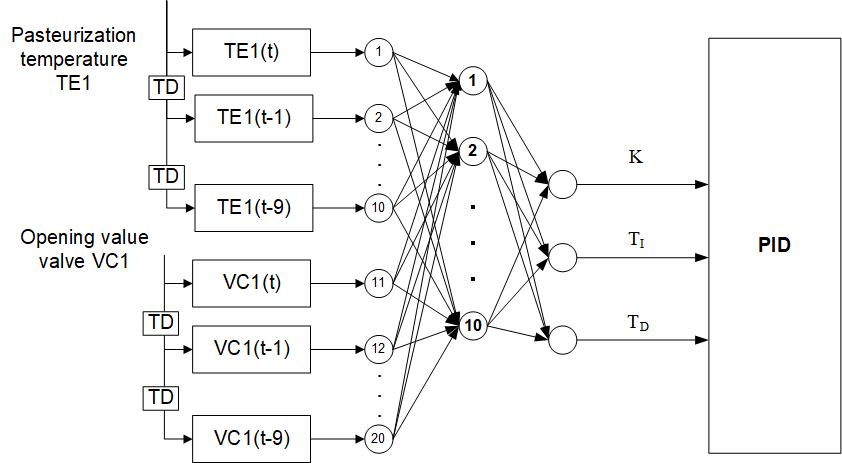
\includegraphics[width=\columnwidth]{figures/Neuro-adjuster-PID.png}
  \caption{PID controller structure}
  \label{fig:pid_controller}
\end{figure}

\section{Examples}

Here are some examples of the application of neuro-symbolic control in various
fields used by Kaspersky \cite{KasperskyMLAD}.

Kaspersky MLAD is designed to predict industrial process data and identify signs
of future anomalies in equipment operation. The goal is to prevent failures,
accidents, and unplanned downtime by detecting warning signs long before they
affect enterprise operations. For Kaspersky, an anomaly is a significant
deviation of actual process data from the forecast.

Kaspersky developed MLAD because existing monitoring systems were outdated,
unable to find the causes of accidents, and overwhelmed by the volume of
telemetry data.

\begin{figure*}[ht]
    \centering
    \thispagestyle{empty}
    % ограничиваем ширину и высоту, сохраняем пропорции
    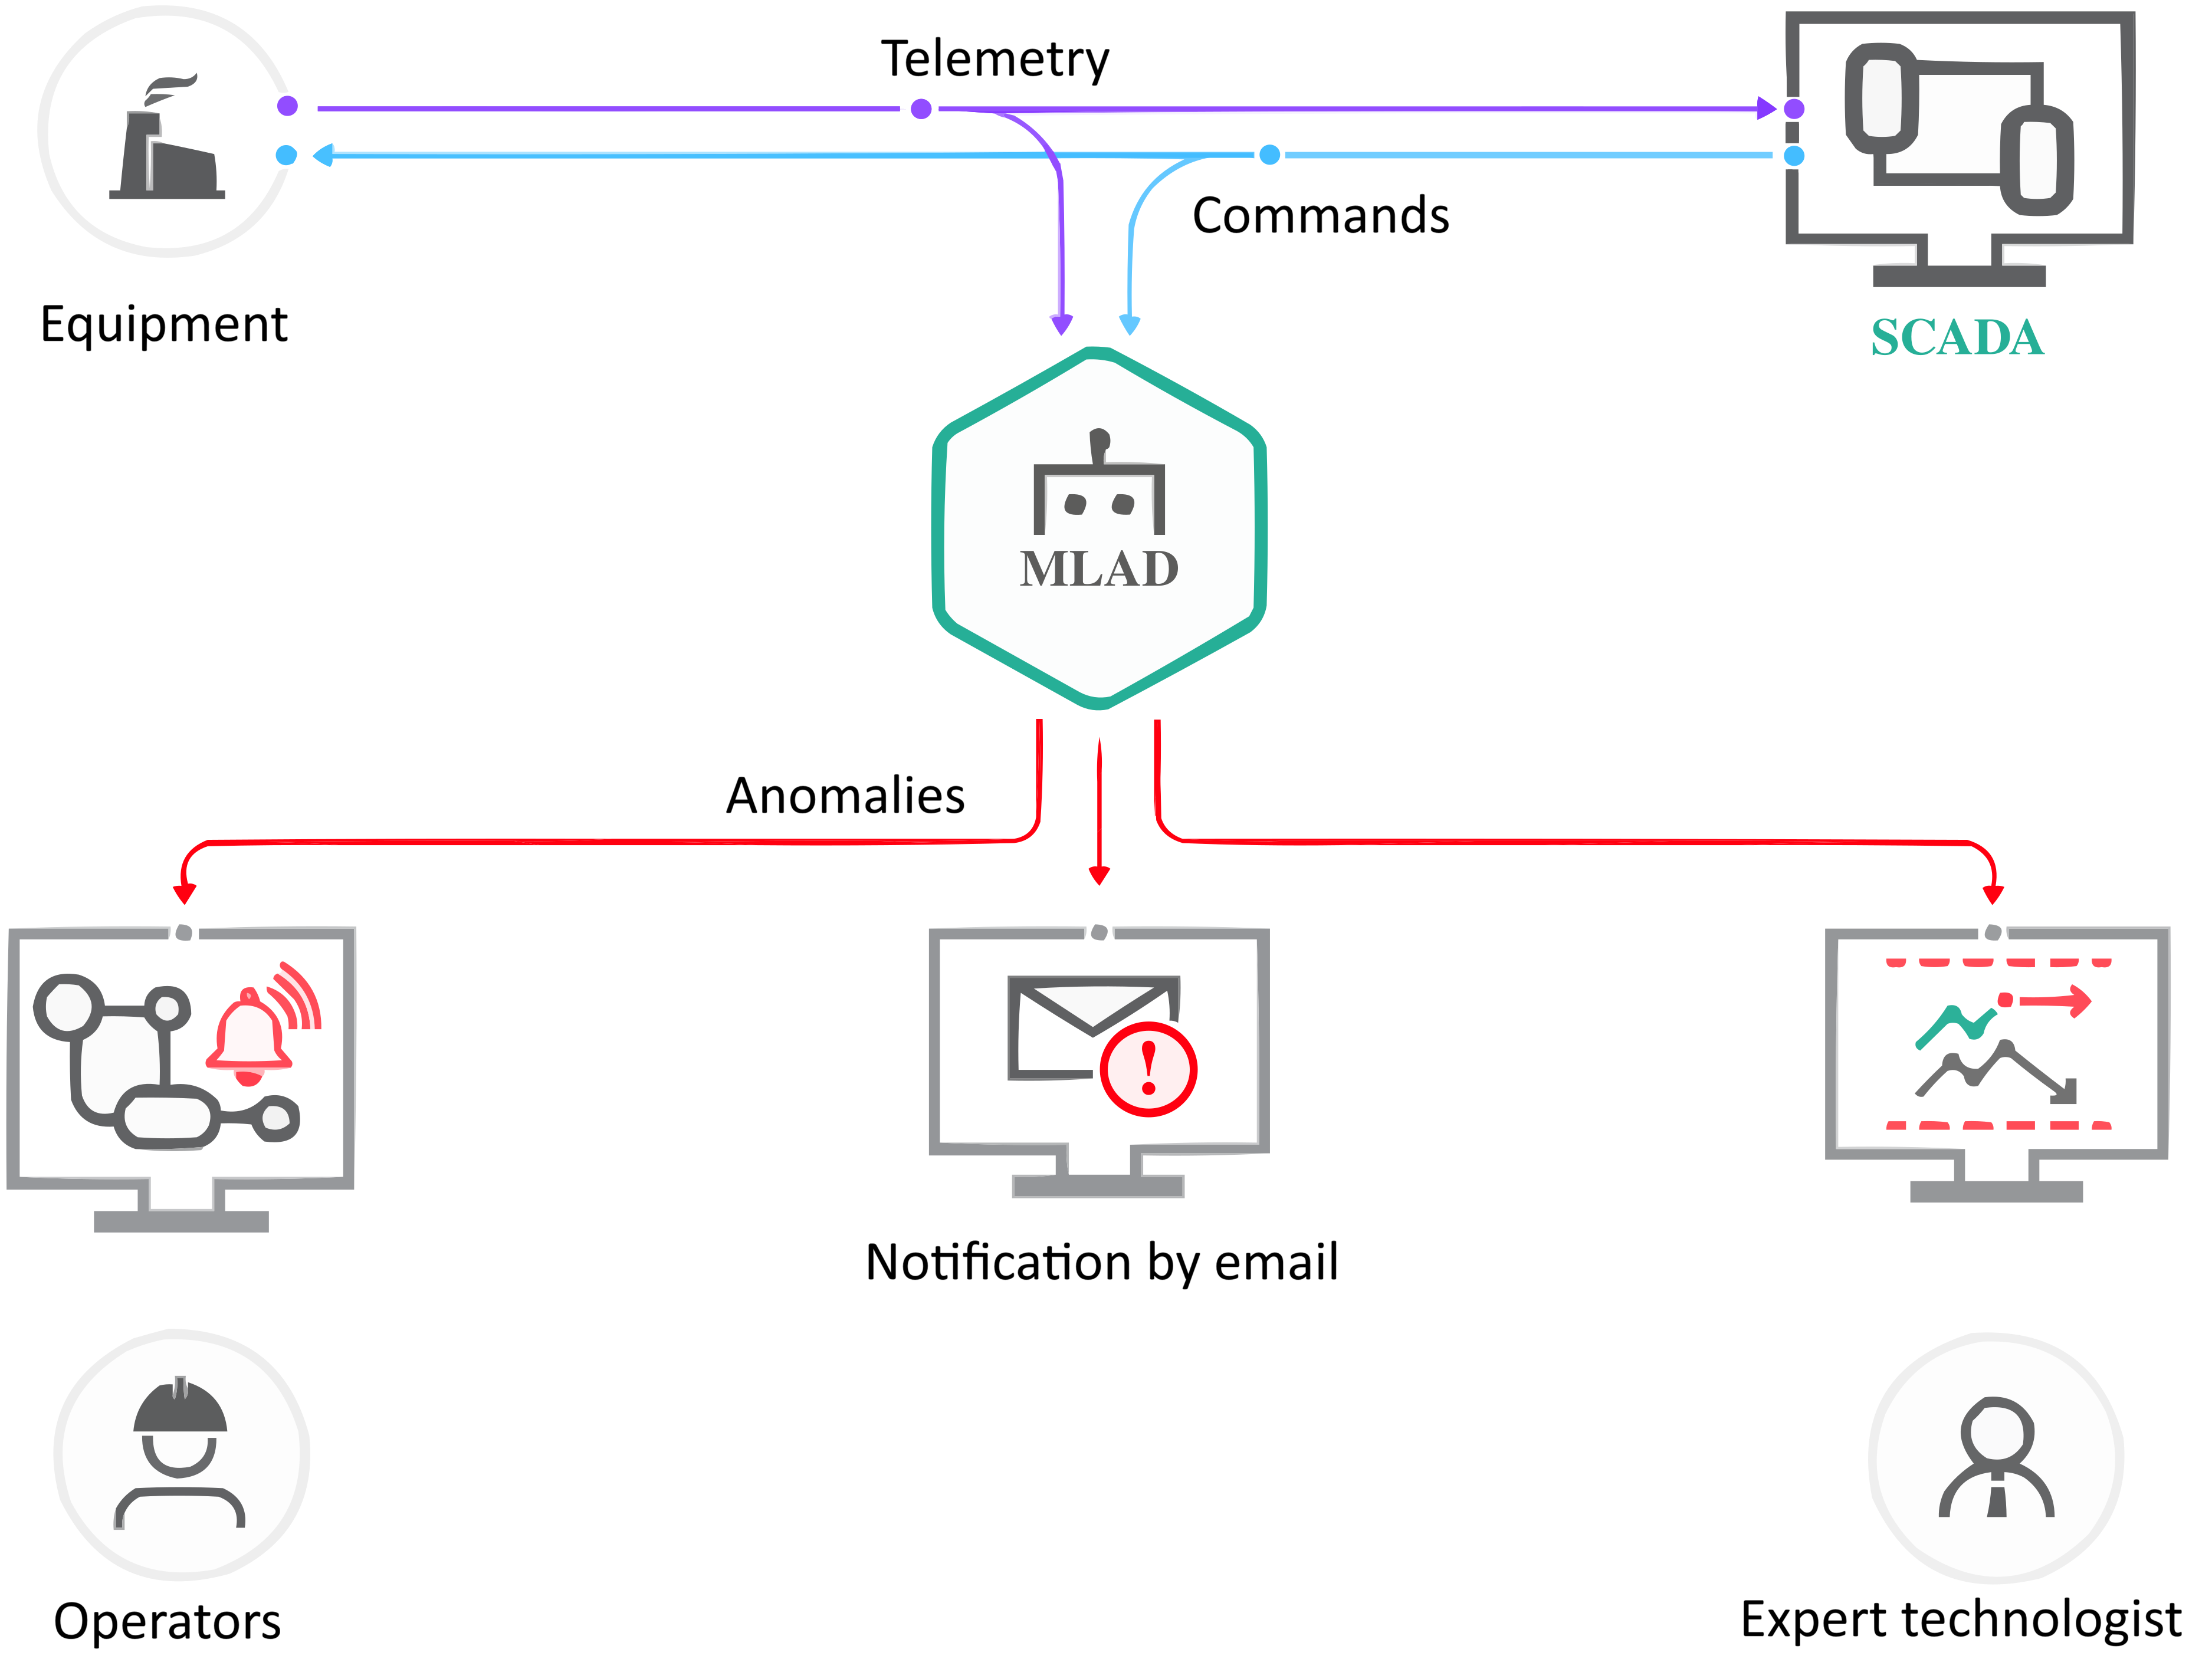
\includegraphics[width=\linewidth, height=0.9\textheight, keepaspectratio]
        {figures/MLAD_in_industry.png}
    \caption{Kaspersky MLAD system in the production process}
    \label{fig:MLAD}
\end{figure*}

Kaspersky MLAD monitors large telemetry streams and identifies deviations that
can threaten production. It predicts process data, detects anomalies, and helps
prevent failures, accidents, and unplanned downtime. The system's place and role
are shown in Fig.~\ref{fig:MLAD}.

The operation of Kaspersky MLAD does not require any modification of the
industrial process. It does not affect the process or interfere with data
transmission or industrial control equipment. The system notifies the operator
about possible failures while leaving the final decision to the operator.

From a technical perspective, Kaspersky MLAD uses neural networks to analyze
telemetry streams. Because telemetry parameters are interconnected and influence
each other, the system identifies relationships between parameters and uses them
to build a forecast. This forecast is then processed by various neuro-semantic
means to reveal anomalies.

Kaspersky MLAD uses various neural network architectures such as CNN, DenseNet,
TCN, and RNN. The first three architectures are used for different kinds of data
processing, analysis, and anomaly detection, while RNNs forecast industrial
process data. Thus, Kaspersky MLAD consists of different neural network modules
interacting with each other.

But how exactly does the Kaspersky MLAD system detect anomalies? For this, the
system has six types of anomaly detectors, or more precisely, analytical
processors:

\begin{itemize}
    \item predictive detector;
    \item state classifier;
    \item rule-based diagnostic detector;
    \item time-to-threshold forecast detector;
    \item stream processor;
    \item event processor.
\end{itemize}

The predictive anomaly detector is a system that first predicts the current
values of an object’s parameters, after which the prediction is compared with
the actually observed behavior. If the deviation between the real process
behavior and the predicted behavior is significant, then the predictive detector
classifies it as an anomaly. The detector is trained on historical telemetry
data and detects anomalies “without hints” from an expert — including previously
unknown anomalies that nobody has noticed.

The state classifier uses Gaussian models, or more precisely, the “elliptical
envelope” algorithm. This detector is used for automatic detection of object
states that differ significantly from the states corresponding to normal
operating modes.

The rule-based diagnostic detector is used to detect anomalies whose symptoms
are known in advance. The detector monitors changes in the object’s behavior
according to specified criteria. Any verification logic can be implemented in
the diagnostic rules. The most popular criteria are: persistent threshold
exceedance, increase or decrease of a metric over a period, step changes, and
“freezing” of values at one level.

The time-to-threshold forecast detector is also used to predict when a
particular technological parameter will reach a certain threshold value. The
detector triggers when the time remaining to the threshold is less than
specified in the settings.

The stream processor brings the real-time telemetry data arriving from the
monitored object to an equal-interval time grid required for the operation of
predictive detectors and diagnostic rules. In the process of converting data to
an equal-interval time grid, the stream processor identifies and, as far as
possible, eliminates stream defects such as data loss, receiving invalid values,
and observations arriving too early or too late.

Unlike the predictive detector, which analyzes continuous time series, the event
processor works with sequences of discrete events. A special type of neural
network analyzes the event stream, identifying typical patterns. An anomaly in
this case is an unusual sequence of events, for example, personnel actions
and/or a series of anomalies detected by other detectors.

\begin{figure*}[ht]
    \centering
    \thispagestyle{empty}
    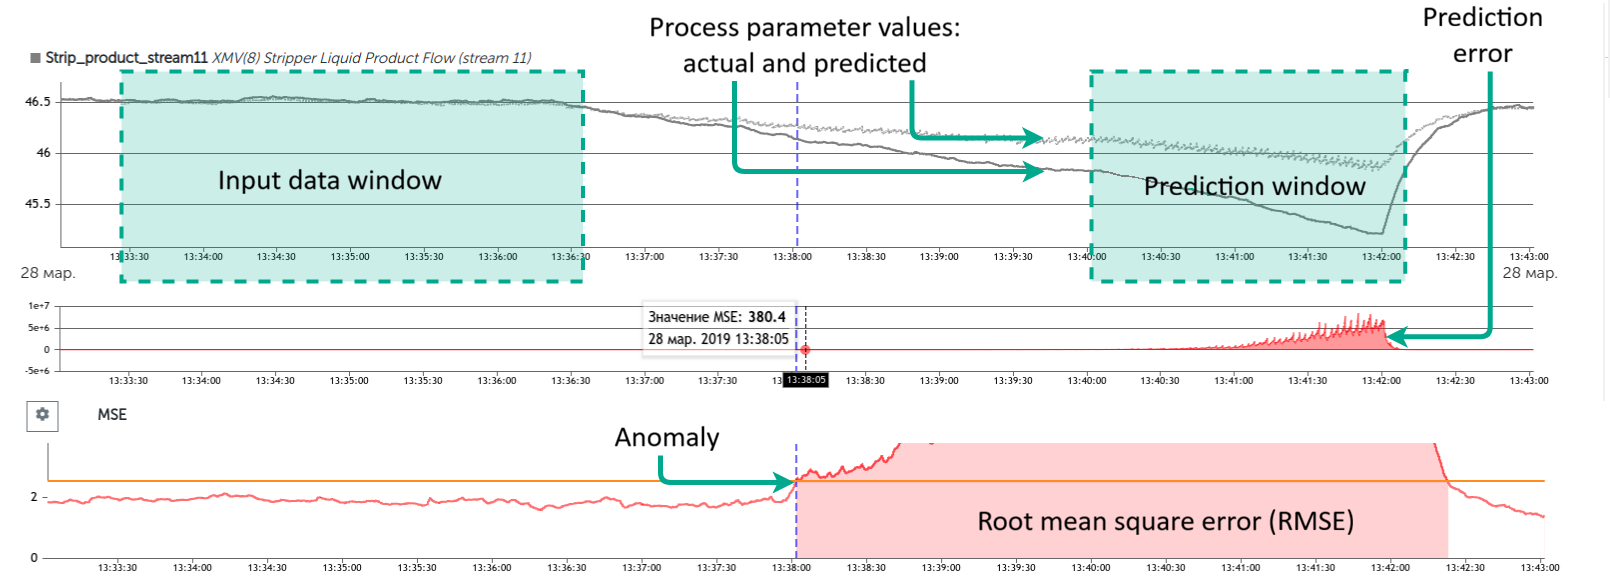
\includegraphics[width=\linewidth]{figures/MLAD_example.png}
    \caption{Example of the operation of the Kaspersky MLAD predictive detector}
    \label{fig:MLADex}
\end{figure*}

Among all the detector types, it is worth focusing in more detail on the
predictive detector. Its operation is simple: first a data forecast is made,
then this forecast is compared with the actually observed behavior, and
anomalies are determined using machine learning. This module can be divided into
two models: a forecasting model and a forecast processing model. The predictive
detector is needed to analyze technological process data, mainly presented as
time series containing various information about the object’s state, different
physical quantities taken from sensors, and so on. The predictive detector works
according to a specific algorithm. First, an input data window is formed from
the technological process data arriving at the predictive detector. Based on the
input data window, a forecast is made, forming a prediction window. This window
shows the object’s behavior in the near future. Then the error is calculated
between the forecast and the actually observed data for each predicted value.
Next, the mean squared error is computed from the set of these errors. When
calculating this error, the values of individual forecast errors are multiplied
by specific weights. Thus, the transition to the second neural network model of
the predictive detector is performed. This module determines an anomaly based on
the value of the mean squared error with the help of a certain threshold that is
formed during the training of the neural network model. An example of this
process can be seen in Figure \ref{fig:MLADex}.

\subsection{Amazon}

After the explosive debut of ChatGPT in 2022, the world of artificial
intelligence became obsessed with neural networks. Giant language models trained
on trillions of words became a symbol of progress — and at the same time a
source of concern because of their “black box”: systems generate plausible
answers but cannot explain why they arrived at that conclusion. Recent analysis
of modern LLMs, including discussions around O3 and Grok 4, highlights both
their emerging utility and the continuing need for transparent, controllable AI
systems \cite{Marcus2024}. A similar review in \textit{The Wall Street Journal}
shows how Amazon uses a neuro-symbolic approach to increase the interpretability
and reliability of neural networks \cite{WSJ2024}.

However, as \textit{The Wall Street Journal} reminds us, neural networks are not
the only path in AI. An approach that was temporarily forgotten, known as
symbolic reasoning, is attracting attention again. Unlike statistical models, it
relies on logic, rules, and explicitly defined symbols, allowing machines to
solve problems that can be formalized as code or mathematical statements.

This is how Amazon presented a way to use the neuro-symbolic approach for its
purposes. The new approach combines the power of modern neural networks (such as
LLMs) with classical symbolic reasoning methods such as logic, rules, and
automated theorem proving. This Amazon approach allows systems not only to
“guess” answers based on statistics, but also to reason soundly, verify the
correctness of their conclusions, and operate with much smaller volumes of data
compared to purely neural approaches.

It is this hybrid — neuro-symbolic AI — that combines the intuition of neural
networks with the rigor of logic — that is considered a promising direction.
Amazon has hinted that this technology can be applied not only to application
software, but also to the control of complex physical systems such as robots.
For example, the robotic arm \textit{Vulcan} (Amazon warehouse automation
systems) shows that the company can use such methods to improve the reliability
of autonomous systems where mistakes are unacceptable.

Beyond robots, Amazon is actively advancing in the software world as well.

In 2025, \textit{Amazon Web Services (AWS)} continues to develop its cloud
services, offering innovative solutions for various industrial sectors. One of
the key directions is the integration of artificial intelligence and machine
learning into production automation and supply chain management processes.

In particular, AWS uses neuro-symbolic agents for:

\begin{itemize}
    \item increasing safety and explainability in regulated industries (for
    example, finance, healthcare), where it is critically important to
    understand why an AI made a particular decision.
    \item automating complex tasks that require logical inference: processing
    documents up to 80,000 tokens, analyzing regulations, verifying code, and
    making rule-based decisions.
    \item reducing computing costs: by integrating symbolic methods, it is
    possible to reduce dependence on huge volumes of data and parameters, making
    systems more efficient and environmentally friendly.
\end{itemize}

In addition, Amazon supports research in this area through programs such as the
\textit{Automated Reasoning Call for Proposals} (autumn 2025), aimed at
developing “sound neuro-symbolic reasoning” that combines language models,
automated solvers, and proof checking to improve the efficiency of solving
complex tasks.

\subsection{Humanoid robot Unitree G1 (China)}

In 2025, a hybrid approach combining the advantages of neural methods and
symbolic (logical) systems — the so-called neuro-symbolic control — is gaining
increasing traction in autonomous robotics. One example of implementing this
technology is humanoid robots such as \textit{Unitree G1}, developed by the
Chinese company \textit{Unitree Robotics}. This robot, presented as a platform
for research and potential commercial use, demonstrates high mobility, balance,
and the ability to perform complex manipulations. However, to perform tasks in
dynamic, partially observable, and unstructured environments (for example, in
everyday life or in production), not only low-level motion control is required,
but also the ability to reason, plan, and interpret context — this is precisely
where the value of the neuro-symbolic approach becomes apparent.

The main goal of introducing neuro-symbolic control into \textit{Unitree G1} has
been to overcome the limitations of purely neural systems, which, despite their
high effectiveness in pattern recognition and motion control, lack
interpretability, generalize poorly to new scenarios, and are not capable of
logical inference. At the same time, classical symbolic systems — based on
rules, ontologies, and logical inference — are too rigidly structured and do not
cope with noise, uncertainty, and the variability of the real world. The
neuro-symbolic approach combines the flexibility of learning from data with
structured decision logic.

The control system of \textit{Unitree G1} in 2025 is implemented as a
multi-level hybrid architecture consisting of:

\begin{enumerate}
    \item \textbf{Perceptual level} — based on deep neural networks (Vision
    Transformers, 3D CNN, PointNet++), responsible for processing data from
    cameras, lidars, IR sensors, and tactile sensors. This level is responsible
    for object detection, gesture recognition, and pose estimation of a person
    and other agents.
    \item \textbf{Symbolic level} — implemented using domain ontologies and
    logical programming languages (for example, Answer Set Programming or
    Probabilistic Soft Logic). Here knowledge about the world is formalized: “a
    cup is on the table”, “the door is closed”, “a person asks to bring water”.
    This level allows building causal chains and checking the consistency of
    states.
    \item \textbf{Interface module} — a neuro-symbolic translator that converts
    continuous outputs of neural networks into discrete symbolic assertions and,
    conversely, uses symbolic plans to generate target trajectories or commands
    for low-level controllers. Differentiable logic layers (for example, Neural
    Logic Machines) and knowledge encoders based on large language models (LLMs)
    fine-tuned on technical and everyday scenarios play a key role here.
    \item \textbf{Action planner} — a hybrid module combining classical planning
    (PDDL, HTN) with reinforcement learning (PPO, SAC). It generates a sequence
    of actions that takes into account both the physical constraints of the
    robot and the logical conditions for task execution.
\end{enumerate}

Although by 2025 \textit{Unitree Robotics} has not officially announced the
introduction of neuro-symbolic control in \textit{G1}, the platform’s
architecture — including an open SDK, ROS 2 support, multimodal sensors, and
integration with large models (for example, UnifoLM) — makes it a promising
basis for implementing such hybrid systems. Approaches that could potentially be
adapted for G1 are actively being studied in the scientific community.

\section{PLCnext and AXC F 2152}

The neural network will be deployed on PLCnext controllers.

PLCnext Control is the hardware platform of PLCnext technology, providing an
open Linux environment with access to more data through Internet of Things
systems and greater flexibility. In addition to standards such as IEC 61131,
parallel programming and a combination of programming languages such as C/C++,
C\#, or MATLAB® Simulink® are also possible in real time with PLCnext Control.
There are three different categories of PLCnext control: flexible modular
controllers, high-performance remote field controllers, and iPC-based
controllers.

The advantages of the PLCnext platform, together with the chosen deployment
method, make it possible to effectively apply the developed neural network.

In this project, the PLCnext Technology Starterkit is used as the control device
(see Figure \ref{fig:ACXF2152}). This kit includes everything needed to work
with PLCnext technology for industrial automation. The kit contains the control
device — an \textbf{AXC F 2152} controller — AXL Smart Elements DI16/DO16/AI4
I/O modules, a slide potentiometer, an Ethernet cable, a starter kit manual, and
a link to a modeling file. The kit is designed to provide a simple, convenient,
and cost-effective way to start projects using PLCnext technology. With this
kit, users can test the operation, control, and high performance of PLCnext
technology on a compact station. The PLCnext Starterkit comes with detailed
documentation and a user manual that help developers get started quickly. It can
also provide access to online courses and materials for additional training and
deepening knowledge of PLCnext.

\begin{figure}[ht]
    \centering
    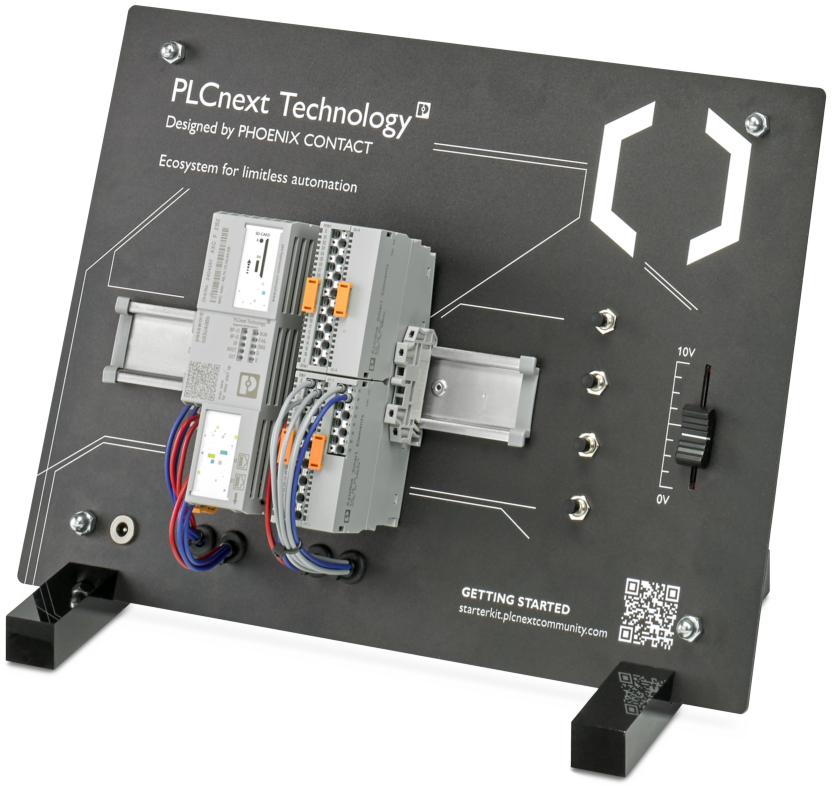
\includegraphics[width=0.45\textwidth]{figures/plcnext_x.png}
    \caption{PLCnext Technology Starterkit}
    \label{fig:ACXF2152}
\end{figure}

Let us now look in more detail at the “heart” of the platform — the AXC F 2152
controller. The controller has powerful computing capabilities, various I/O
interfaces, and support for multiple programming languages.

Detailed technical specifications of the \textbf{AXC F 2152}:

\begin{itemize}

    \item[-] Processor:
        \begin{itemize}
            \item[•] CPU: dual-core ARM Cortex-A9.
            \item[•] Processor frequency: 800 MHz.
            \item[•] Built-in memory: 1 GB RAM, 4 GB eMMC.
        \end{itemize}

    \item[-] Communication interfaces:
        \begin{itemize}
            \item[•] Ethernet: 2 x 10/100/1000 Mbps.
            \item[•] USB: 2 x USB 2.0 Host.
            \item[•] RS232: 1 x port with RTS/CTS support.
        \end{itemize}

    \item[-] Inputs/outputs:
        \begin{itemize}
            \item[•] Digital inputs: 16 x 24 V DC, with counter support.
            \item[•] Digital outputs: 16 x 24 V DC, maximum current 500 mA per
            output.
            \item[•] Analog inputs: 2 x 0-10 V, 12-bit resolution.
            \item[•] Analog outputs: 2 x 0-10 V, 12-bit resolution.
        \end{itemize}

    \item[-] Expansion:
        \begin{itemize}
            \item[•] Expansion slots: 2 x PLCnext expansion module slots.
            \item[•] Support for expansion modules: I/O modules, communication
            interface modules, and additional functional modules.
        \end{itemize}

    \item[-] Power:
        \begin{itemize}
            \item[•] Supply voltage: 24 V DC.
            \item[•] Power consumption: up to 18 W.
        \end{itemize}

    \item[-] Operating system:
        \begin{itemize}
            \item[•] PLCnext Runtime: based on Linux.
        \end{itemize}

    \item[-] Software:
        \begin{itemize}
            \item[•] Supported programming languages: IEC 61131-3 (ST, LD, FBD,
            SFC), C++, C\#, Python.
            \item[•] Built-in software: PLCnext Engineer, PLCnext Runtime.
        \end{itemize}

    \item[-] Operating conditions:
        \begin{itemize}
            \item[•] Operating temperature: 0°C to 55°C.
            \item[•] Humidity: 5\% to 95\%, non-condensing.
        \end{itemize}

\end{itemize}

The main components of the \textbf{AXC F 2152} (modules, interfaces) are shown
in Figure \ref{fig:PLCComplect}.

\begin{figure}[ht]
    \centering
    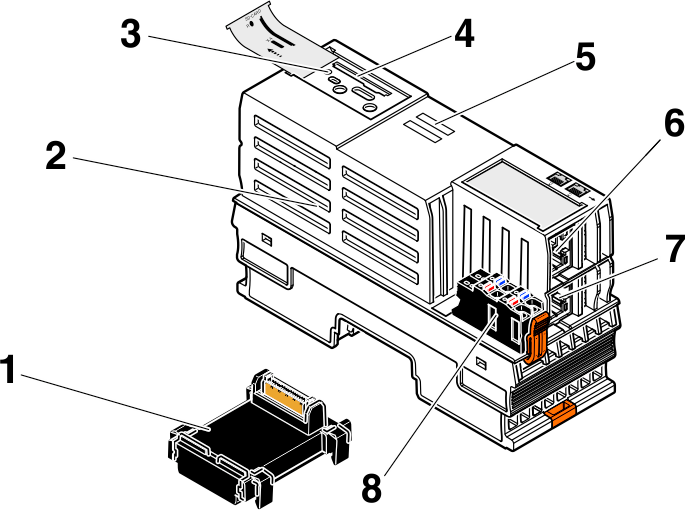
\includegraphics[width=0.45\textwidth]{figures/plcnext_complect.png}
    \caption{Components of the \textbf{AXC F 2152}}
    \label{fig:PLCComplect}
\end{figure}

The controller includes:

\begin{enumerate}
    \item Basic bus module.
    \item Electronics module.
    \item Reset button.
    \item SD cardholder.
    \item Diagnostic and status indicators.
    \item Ethernet interface (1).
    \item Ethernet interface (2).
    \item Power connector.
\end{enumerate}

To connect various peripherals to the \textbf{AXC F 2152}, the following steps
must be taken:

\begin{enumerate}
    \item Use the base bus module to connect the controller to the Axioline F
    local bus, which can support up to 63 I/O devices.
    \item Use the Ethernet interface(s) to connect the controller.
    \item Configure the network and controller settings.
    \item Create a new project, add the controller and peripheral devices to the
    hardware configuration.
    \item Download the project to the controller and start it.
\end{enumerate}

Various Axioline F I/O devices can be connected to the \textbf{AXC F 2152}, such
as:

\begin{itemize}
    \item[-] Digital I/O modules (for example, DI8/1 DO8/1 2701916) for handling
    discrete signals.
    \item[-] Analog I/O modules (for example, AI2 AO2 2702072) for handling
    analog signals.
    \item[-] Special-purpose modules (for example, AXF BK PN 2701815) for
    connection to other buses.
\end{itemize}

The AXC F 2152 PLCnext Control controller has high performance, a variety of
communication interfaces, scalability, and support for multiple programming
languages. It is well suited for process automation, offering flexibility,
reliability, and ease of development.

\subsection{Development with PLCnext}

The neural network was developed on Windows using Visual Studio 2022. To deploy
on PLCnext controllers, these projects must be built for the target platform.

Visual Studio is a powerful and popular integrated development environment (IDE)
from Microsoft. The following advantages led to choosing it as the most suitable
tool for the project:

\begin{itemize}

    \item[-] Rich functionality. Visual Studio Community provides a wide range
    of tools and capabilities for developing and debugging software. It supports
    various programming languages, including C++, C\#, Visual Basic, Python, and
    others that can be used with the PLCnext SDK. Visual Studio also includes
    tools for debugging, profiling, version control, and automation.

    \item[-] Integration with other tools. Visual Studio Community integrates
    with various development services and tools, which simplifies working with
    them. Visual Studio includes the PLCnext Technology Development Tools
    extension, which adds project templates and elements, as well as a debugging
    module for PLCnext Technology. VS also supports CMake, which is the build
    system for this project.

    \item[-] Availability. Visual Studio Community is free for non-commercial
    use, including academic and personal projects. This helps reduce licensing
    costs for the development environment.

\end{itemize}

PLC Toolchain will be used for programming the controller. It is a set of tools
for programming logic controllers in high-level languages such as C++ and C\#.
It enables the use of these languages to create complex, efficient control
algorithms and to integrate with other systems and technologies.

PLC Toolchain is based on the \textbf{Beremiz} development environment, which
complies with the IEC 61131-3 standard. This standard defines five programming
languages for PLCs: Instruction List, Symbolic Flowchart, Ladder Diagram,
Function Block Diagram, and Structured Text. PLC Toolchain allows these
languages to be used in combination with C++ and C\#, and also supports code
portability across different platforms and hardware.

PLC Toolchain includes tools for creating Human-Machine Interfaces (HMIs) and
for connecting PLC programs to existing databases and fieldbuses.

The PLCnext SDK is also required to work with the PLCnext platform and the AXC F
2152 controller. It is a set of tools for developing applications for PLCnext
Technology controllers in different programming languages. The PLCnext SDK
includes compilers, debuggers, libraries, and other resources needed to create
native applications for the target device. PLCnext SDK is installed and managed
via the command line interface (CLI) called PLCnext CLI, or \textbf{plcncli}.

\subsection{Installation of PLCnext}

After the neural network has been built, the resulting executable needs to be
transferred to the existing controller.

For this task, several options can be used:

\begin{itemize}
    \item[-] WinSCP combined with PuTTY 64-bit.
    \item[-] Specialized PLCnext Engineer software tools.
\end{itemize}

These tools each have their own advantages and disadvantages. Let us describe
them.

The main advantage of PLCnext Engineer is that it is specifically tailored to
the PLCnext technology. PLCnext Engineer is an engineering suite for developing
automated solutions based on controllers. It includes all the engineering
disciplines necessary for the full development and commissioning of an
automation project. These engineering tasks include:

\begin{enumerate}
    \item Network configuration.
    \item Development of application code.
    \item HMI (Human-Machine Interface).
    \item OPC UA server.
\end{enumerate}

These functions make PLCnext Engineer a highly suitable tool for deploying the
developed program to the controller.

However, PLCnext Engineer is not the only alternative. To make an informed
choice, it is worth considering other tools such as PuTTY combined with WinSCP.

PuTTY is an SSH and telnet client originally developed by Simon Tatham for the
Windows platform. PuTTY is open-source software, available with source code and
maintained by a group of volunteers.

WinSCP is a free open-source SFTP client, FTP client, WebDAV client, S3 client,
SCP client, and file manager for Windows. Its primary function is file transfer
between local and remote computers. In addition, WinSCP provides scripting and
basic file manager features.

WinSCP provides:

\begin{itemize}
    \item[-] A graphical user interface.
    \item[-] Support for multiple languages.
    \item[-] Integration with Windows (drag-and-drop, URLs, quick access icons,
    navigation history).
    \item[-] Common file operations for both local and remote files.
    \item[-] Support for SFTP and SCP over SSH, as well as FTP, WebDAV, and S3.
    \item[-] A scriptable command-line interface and .NET assembly for advanced
    programming tasks.
    \item[-] Directory synchronization using several semi-automatic modes.
    \item[-] A built-in text editor.
    \item[-] Shared site storage with PuTTY.
    \item[-] Authentication support using password, keyboard-interactive, public
    key, and Kerberos (GSS).
    \item[-] Integration with Pageant (PuTTY authentication agent) for full SSH
    public key authentication support.
    \item[-] A file explorer and interface manager.
    \item[-] Optional protection of saved site information with a master
    password.
    \item[-] Optional portable mode using a configuration file instead of
    registry entries, suitable for removable media.
\end{itemize}

This choice was made because these programs are simple, highly functional, and
together can cover all necessary requirements for transferring the compiled
neural network executable to the controller.

\subsection{Porting to PLCnext}

The following components will be used to build the program for the controller:

\begin{enumerate}
    \item CMake (build system).
    \item \textbf{plcncli} (command line for PLCnext controllers).
    \item SDK for the selected controller.
\end{enumerate}

To successfully build the program for the selected controller, CMake must be
installed on the computer. This tool provides the ability to perform
cross-platform builds for different targets.

After CMake is installed, the \textbf{plcncli} command line must be installed to
download the selected SDKs and build programs for the target controller. It
provides the necessary build tools.

After \textbf{plcncli} has been installed, you need to download and install the
SDK from the official site using the \textbf{plcncli} command:

\begin{lstlisting}[basicstyle=\ttfamily\small,breaklines=true,breakatwhitespace=true]
plcncli.exe install sdk -d [installation path] -p [path to archive file]
\end{lstlisting}

After the SDK is installed, you need to open Visual Studio and configure the
CMake project for the controller.

\section{Developed Neuro-PID controller}

The overall structure of the self-tuning Neuro-PID controller is shown in Fig.
\ref{fig:neuro_PID_controller}, where the neural network (NN) outputs are
proportional ($K$), integral ($T_I$), and differential ($T_d$) components
\cite{ivaniuk2013neuro}.

\begin{figure*}[ht]
  \centering
  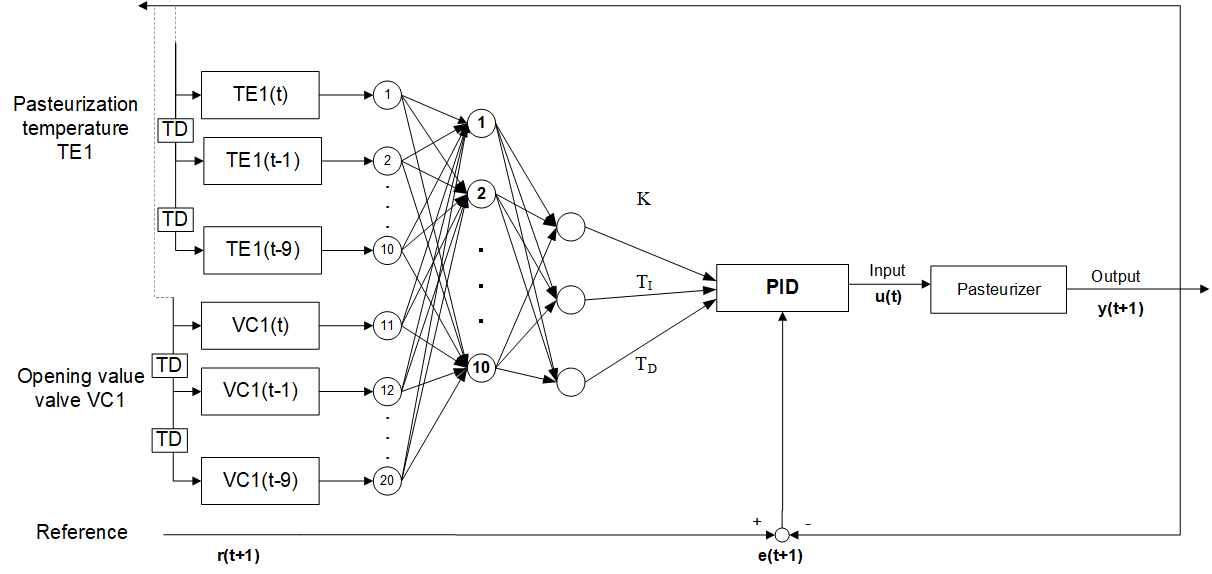
\includegraphics[width=\textwidth]{figures/pic_developed_NN_full.png}
  \caption{The developed Neuro-PID controller (TD means delay operator)}
  \label{fig:neuro_PID_controller}
\end{figure*}

To control the Pasteurizer \cite{ivaniuk2013neuro}, a PID controller is
configured with a multilayer perceptron (MLP, neuro-PID adjuster) with the
following structure: 20 input, 10 hidden and 3 output neural elements; the
activation function for the hidden and output layers is sigmoid.

The discrete-time \textbf{PID controller} can be described by equation
\ref{PID_algorithm} \cite{ivaniuk2013neuro}, where $P$, $T_I$ and $T_D$ are
proportional factors, integral and differential constituents respectively, $u_n$
determines the input of a control object at a time of $t = n T_0$ and $e_n$ — an
error between the desired output value of $r_n$ and the real output of $e_n =
r_n - y_n$. $T_0$ defines a unit time interval.

\begin{equation}\label{PID_algorithm}
  \begin{aligned}
    u_k  & = u_{k - 1} + \Delta u_k,                                         \\
    \Delta u_k & = q_0 e_k + q_1 e_{k - 1} + q_2 e_{k - 2},                  \\
    q_0  & = \mathbf{K}\left(1 + \frac{T_D}{T_0}\right),                     \\
    q_1  & = -\mathbf{K}\left(1 + 2\frac{T_D}{T_0} - \frac{T_0}{T_I}\right), \\
    q_2  & = \mathbf{K}\frac{T_D}{T_0}.
  \end{aligned}
\end{equation}

Algorithm for operation of \textbf{neuro-PID adjuster} \cite{ivaniuk2013neuro}:

\begin{equation}\label{PID_nn}
  \begin{aligned}
    y_j       & = F(\sum_{i}{\omega_{i j}y_i - T_j}),                         \\
    \gamma_j  & = y_j - t_j,                                                  \\
    \gamma_i  & = \sum_{i}{\gamma_iF^\prime(S_i)\omega_{j i}},                \\
    \omega_{i j}(t + 1) & = \omega_{i j}(t) - \alpha\gamma_jF^\prime(S_j)y_i, \\
    T_j(t + 1)& = T_j(t) + \alpha\gamma_jF^\prime(S_j),                       \\
    E         & = \frac{1}{2}\sum_{k = 1}^{L}{\sum_{j}{({y_j}^k} - {t_j}^k)^2}.
  \end{aligned}
\end{equation}

To use the back propagation algorithm, we must select the $E$ function, which
must be minimized. It will be the management error $e_n$ at the time $t = n
T_0$, so $E_n = \frac{1}{2}e_n^2$. To accumulate errors, we store the data we
have previously obtained — $E_{n-p},... E_{n-2},E_{n-1},E_n$, where $p$
determines the number of previously saved images used for network learning
(\ref{PID_nn}).

\section{Examples of system operation with natural language information display}

For information to be clear and understandable to the reader, it must be
presented consistently. The recipe authoring system interface allows the
structure of domains and ontologies to be expressed in natural language. This
process of converting an internal knowledge representation to an external
knowledge representation is performed by a graphical interface component.

\section{Integration of third-party solutions with a knowledge base}

A standard system built on the basis of OSTIS Technology can be easily
integrated with other systems in the workplace. To integrate
\textit{\textbf{ISA-88}}, \textit{\textbf{ISA-95}} and \textit{\textbf{ISA-5.1}}
standards system with other systems running on JSC "Savushkin Pro\-duct", a
web-oriented approach is used — the OSTIS server is accessed with the use of the
following queries:

\begin{lstlisting}[basicstyle=\small]
  http://industry.ostis.net?sys_id=unit
\end{lstlisting}

where "sys\_id=unit" defines a term (the name of an entity) whose value we want
to find out (in this example, in fact, the answer to the question "What is a
\textit{unit}?"). This approach makes it relatively easy to add support for the
knowledge base in current control systems projects; it is enough to indicate the
names corresponding to the entities in the knowledge base within the control
system.

Thus, an interactive intelligent help system for control systems projects is
implemented, allowing employees to work with the control system and ask
questions directly during their tasks.

Another example is the integrated help subsystem within corporate Add-in
\textbf{EasyEPLANner} \cite{EasyEPLANner} for CAD EPLAN. It helps describe
technological objects (Tank, Boiler, etc.), operations, and so on according to
the \textit{\textbf{ISA-88}} standard. The UML-model of EasyEPLANner high-level
objects can be described in OSTIS. The \textbf{PID controller} is at the lower
level — the control module. It can be replaced by the development
\textbf{Neuro-PID controller} with the connections to the units and other
high-level objects.

\section{Use in control systems}

It is very important to quickly and correctly react to different events during
process control, especially critical accidents. However, when we have a complex
distributed system, it is rather complicated and normally requires the help of a
human operator. This may lead to a variety of problems. Thus, using an
OSTIS-based system can help solve the issues described in Fig.
\ref{OSTIS_in_control}. For example, Project \#2 has a valve failure but does
not know what to do. It makes a request to the OSTIS server, which already knows
which projects also use this line (with this valve). The OSTIS server polls the
rest of the projects (projects \#1 and \#2). Each project has information about
which operations are currently active and provides an answer on what to do —
pause the operation, do nothing, etc. After that, the OSTIS server sends back to
Project \#2 an answer with the resulting actions to be used. These actions are
performed automatically, without the need for a human operator.

\begin{figure}[ht]
  \centering
  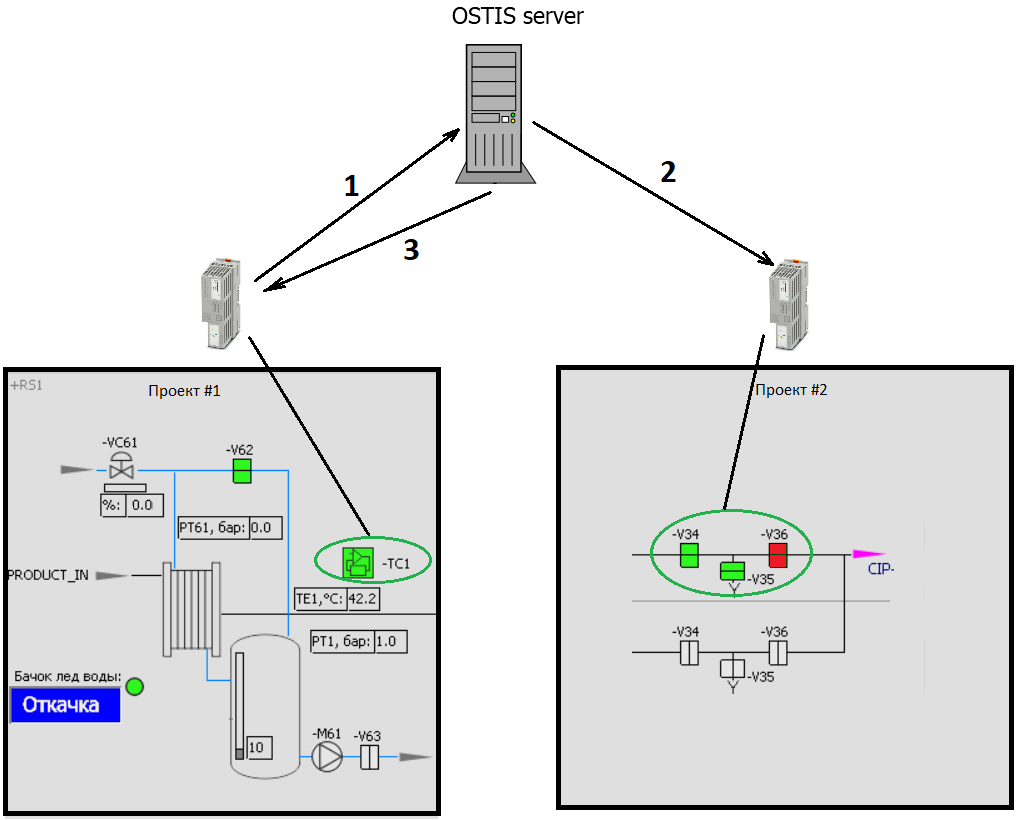
\includegraphics[width=0.45\textwidth]{figures/OSTIS_in_control.png}
  \caption{OSTIS in control systems}
  \label{OSTIS_in_control}
\end{figure}

\section{Future development}

Current project issues can be found on GitHub (\cite{EasyServer_4_0},
\cite{s88-ostis}, and \cite{isa-5.1-ostis}). The main problems to be solved are:
\begin{itemize}
  \item Improving system performance and especially accelerating system response
    time to user requests. This is connected with productivity and overall user
    satisfaction.
  \item Continuously updating and refactoring ontological models (further
    formalization of missing concepts, fixing typos, etc.).
  \item Enhancing PFC-visualization — not only displaying but also editing
    diagrams. Adding rich navigation between PFC-diagrams and corresponding text
    representations.
  \item Further formulation of typical questions to the system from the user and
    their formalization at the level of the existing knowledge base.
  \item Adding detailed descriptions of real control projects based on the
    existing knowledge base.
\end{itemize}

The implementation of answers to complex questions is necessary to make the work
easier not only for process operators but also for maintenance personnel —
instrumentation engineers, mechanics, electricians, etc. Therefore, it is
planned to implement the system's answer to the following type of question: in
what operations of which objects is this actuator used (for example, valve
\textbf{"T1V1"}). This question is very important when a device failure occurs,
and it is necessary to determine the criticality of this situation. For
analysis, it is necessary to compare the time of the accident and the history of
operations. For example, a failure of the mix-proof valve during the line
washing operation and the active product dosing along the other line should lead
to a stop of these operations and stop the preparation of the batch in the
corresponding unit. The operator must report this to the appropriate maintenance
specialist to fix it. After the fault has been eliminated, the operator
continues to perform operations. This is the correct order of events, which is
crucial to avoid mixing detergent and product. If the device malfunction
occurred within the line, which is now inactive, then this situation has a low
priority, does not lead to a halt in operations, and can be addressed later if
the service personnel have available time.

\section{Conclusion}

This paper considers a technique for automating the creation, development, and
use of standards based on OSTIS Technology. Using the example of the
\textit{\textbf{ISA-88}}, \textit{\textbf{ISA-95}}, and
\textit{\textbf{ISA-5.1}} standards implemented at the Savushkin Product
enterprise, it examines the knowledge base structure, the problem solver
features, and the support system user interface for these processes. The
developed system has been shown to integrate easily with other enterprise
systems, serving as a foundation for building an information service system for
employees within the context of Industry 4.0. The approach proposed in this work
not only automates the processes of creating, agreeing on, and developing
standards but also significantly increases the efficiency of applying standards
both manually and automatically.

\section*{Acknowledgment}

The author would like to thank the research teams of the Departments of
Intelligent Information Technologies at the Belarusian State University of
Informatics and Radioelectronics and the Brest State Technical University.

\bibliographystyle{bib/IEEEtran}
\balance
\bibliography{bib/links}

\bigskip
\begin{otherlanguage}{russian}
  \begin{center}
    \large\textbf{Нейро-символическое управление для пастеризационной установки}
    \medskip
    Иванюк Д.С.
  \end{center}

  \small
  В работе рассмотрен онтологический подход к пониманию, интеграции и развитию
  современных подходов к управлению (нейроуправление, большие языковые модели,
  современные международные стандарты) с использованием Технологии OSTIS.
  Уточнены формальные трактовки основных понятий, используемых в стандартах, что
  позволяет упростить описание реальных задач. Также описаны варианты интеграции
  базы знаний в используемые программные средства разработки и сценарии её
  использования непосредственно в системах управления.

\end{otherlanguage}

\medskip
\normalsize
\hfill Received May 15, 2026
\end{document}
